% !TEX program = xelatex
\documentclass[11pt, a4paper]{article}

\usepackage{fontspec}
\usepackage{xetexko}
\usepackage[margin=2cm, top=2.5cm, bottom=2.5cm]{geometry}
\usepackage{graphicx}
\usepackage{booktabs}
\usepackage{tabularx}
\usepackage{xcolor}
\usepackage{hyperref}
\usepackage{titlesec}
\usepackage{fancyhdr}
\usepackage{enumitem}
\usepackage{float}
\usepackage{caption}
\usepackage{array}
\usepackage{colortbl}
\usepackage{tikz}

\setmainfont{Apple SD Gothic Neo}
\setsansfont{Apple SD Gothic Neo}
\setmonofont{Menlo}

\definecolor{darkblue}{HTML}{1A5276}
\definecolor{medblue}{HTML}{2980B9}
\definecolor{lightblue}{HTML}{D4E6F1}
\definecolor{darkgray}{HTML}{2C3E50}
\definecolor{green}{HTML}{27AE60}
\definecolor{orange}{HTML}{E67E22}
\definecolor{red}{HTML}{E74C3C}
\definecolor{lightgray}{HTML}{F2F3F4}

\hypersetup{colorlinks=true, linkcolor=darkblue, urlcolor=medblue}

\titleformat{\section}
  {\Large\bfseries\color{darkblue}}{\thesection.}{0.5em}{}
  [\vspace{-0.5em}\textcolor{medblue}{\rule{\textwidth}{0.5pt}}]
\titleformat{\subsection}
  {\large\bfseries\color{darkblue}}{\thesubsection}{0.5em}{}

\pagestyle{fancy}
\fancyhf{}
\fancyhead[L]{\small\color{darkgray}AI 기반 리테일 매출·수요 예측}
\fancyhead[R]{\small\color{darkgray}한양대 빅데이터마케팅 랩}
\fancyfoot[C]{\small\color{darkgray}\thepage}
\renewcommand{\headrulewidth}{0.4pt}

\newcolumntype{L}[1]{>{\raggedright\arraybackslash}p{#1}}
\newcolumntype{C}[1]{>{\centering\arraybackslash}p{#1}}

\begin{document}

% ═══════════════════════════════════════════════════════
% COVER
% ═══════════════════════════════════════════════════════
\thispagestyle{empty}
\begin{center}
\vspace*{2.5cm}

{\fontsize{30}{36}\selectfont\bfseries\color{darkblue}
어떤 품목이, 어떤 매장에서,\\[10pt]
얼마나 팔릴지 미리 압니다.}

\vspace{1cm}

{\Large\color{darkgray}
AI 기반 매출·수요 예측 — 폐기 감소, 위험 매장 탐지, 채널 최적화}

\vspace{1cm}
\textcolor{medblue}{\rule{10cm}{0.8pt}}

\vspace{2cm}

\begin{tikzpicture}
\node[fill=lightblue, rounded corners=8pt, minimum width=15cm, minimum height=3cm] {
  \begin{minipage}{14cm}
  \centering
  \vspace{4pt}
  \begin{minipage}[t]{0.3\textwidth}\centering
    {\fontsize{30}{34}\selectfont\bfseries\color{darkblue}98\%}\\[4pt]
    {\normalsize\color{darkgray}매출 예측 정확도}
  \end{minipage}\hfill
  \begin{minipage}[t]{0.3\textwidth}\centering
    {\fontsize{30}{34}\selectfont\bfseries\color{green}284개}\\[4pt]
    {\normalsize\color{darkgray}매장 동시 예측}
  \end{minipage}\hfill
  \begin{minipage}[t]{0.3\textwidth}\centering
    {\fontsize{30}{34}\selectfont\bfseries\color{darkblue}품목별}\\[4pt]
    {\normalsize\color{darkgray}카테고리 단위 수요 예측}
  \end{minipage}
  \vspace{4pt}
  \end{minipage}
};
\end{tikzpicture}

\vspace{3cm}

{\large\color{darkgray}
한양대학교 경영대학\\[4pt]
빅데이터마케팅 랩 · 임보람 교수\\[8pt]
brlim@hanyang.ac.kr\\[4pt]
bigdatamarketinglab.com}

\end{center}

\newpage

% ═══════════════════════════════════════════════════════
% 1. 할 수 있는 것
% ═══════════════════════════════════════════════════════
\section{AI 매출 예측으로 할 수 있는 것}

매장별 매출 데이터가 있으면, AI는 단순히 ``내일 매출이 얼마인지'' 맞추는 것을 넘어서 \textbf{운영 전반의 의사결정}을 바꿀 수 있습니다.

\vspace{0.5cm}

\begin{table}[H]
\centering
\renewcommand{\arraystretch}{1.5}
\begin{tabularx}{\textwidth}{C{0.8cm} L{5cm} X}
\toprule
\rowcolor{lightblue} & \textbf{할 수 있는 것} & \textbf{왜 중요한가} \\
\midrule
\textbf{1} & \textbf{품목별 수요 예측} & 유제품, 신선식품, 베이커리 등 카테고리별로 수요를 예측합니다. 수요를 알면 발주량이 정밀해지고, \textbf{식품 폐기가 줄어듭니다.} \\[6pt]
\textbf{2} & \textbf{매장 위험 조기 탐지} & 매출이 서서히 떨어지는 매장을 \textbf{수개월 전에} 감지합니다. 특정 품목의 판매량이 줄기 시작하면 그것이 전체 매출 하락의 선행 신호입니다. \\[6pt]
\textbf{3} & \textbf{원인 분석} & 매출이 떨어졌을 때, 그것이 경쟁사 때문인지, 고객 변화인지, 계절 요인인지를 \textbf{AI가 분리해서 알려줍니다.} \\[6pt]
\textbf{4} & \textbf{채널별 맞춤 전략} & 온라인 고객과 오프라인 고객은 의사결정 방식이 다릅니다. 채널별로 어떤 수준의 품목 관리가 효과적인지를 데이터로 보여줍니다. \\
\bottomrule
\end{tabularx}
\end{table}

\newpage

% ═══════════════════════════════════════════════════════
% 2. 품목별 수요 예측 → 폐기 감소
% ═══════════════════════════════════════════════════════
\section{품목별 수요 예측 → 폐기율 감소}

리테일에서 가장 큰 비용 손실 중 하나는 \textbf{식품 폐기}입니다. 유제품, 신선식품, 베이커리는 유통기한이 짧아서, 수요 예측이 틀리면 그대로 버려집니다.

AI가 카테고리별 수요를 예측하면, \textbf{발주량을 수요에 맞출 수 있습니다.}

\begin{figure}[H]
\centering
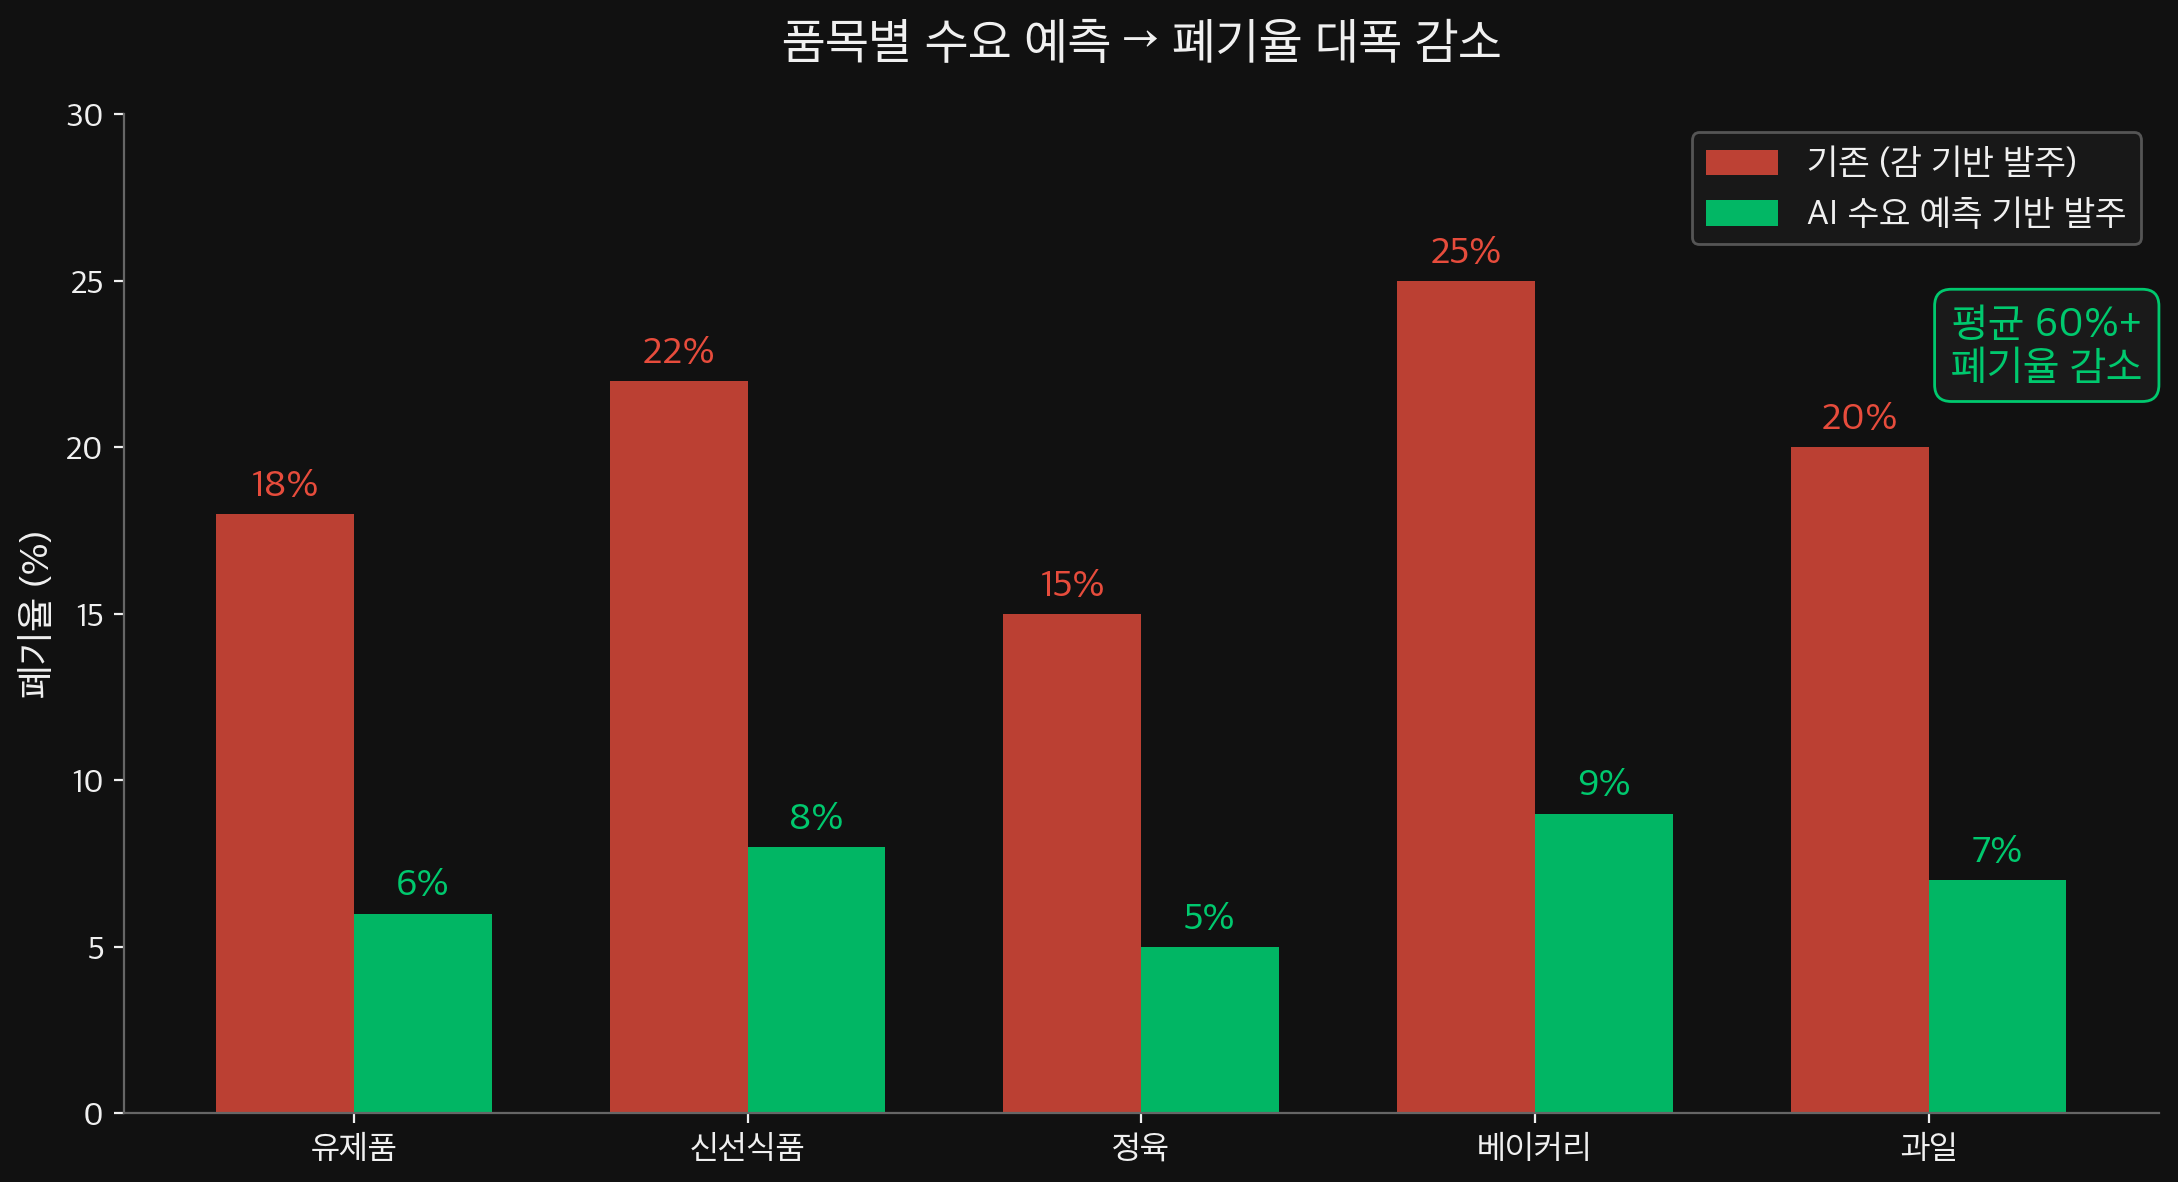
\includegraphics[width=0.85\textwidth]{v2_waste_reduction.png}
\caption{품목별 수요 예측 기반 발주 시 예상 폐기율 감소 (개념도)}
\end{figure}

\colorbox{lightblue}{%
\begin{minipage}{0.95\textwidth}\vspace{8pt}
\textbf{핵심:} 카테고리별로 ``다음 주에 이 매장에서 유제품이 얼마나 팔릴지''를 알면, 발주 단위가 바뀝니다. 과잉 발주로 인한 폐기, 과소 발주로 인한 기회 손실 — 양쪽 모두 줄어듭니다.
\vspace{8pt}
\end{minipage}%
}

\vspace{0.5cm}

실제로 284개 슈퍼마켓 매장 데이터를 분석한 결과, AI 모델은 \textbf{카테고리 수준의 구매 패턴}을 정밀하게 학습합니다. 고객이 어떤 카테고리 상품을 몇 가지 샀는지, 장바구니 구성이 어떤지가 매출을 결정하는 가장 강력한 변수였습니다.

\newpage

% ═══════════════════════════════════════════════════════
% 3. 매장 위험 조기 탐지
% ═══════════════════════════════════════════════════════
\section{매장 위험 조기 탐지}

매출이 떨어지는 매장을 \textbf{실적이 나빠진 다음에} 발견하면 이미 늦습니다.

AI 예측 모델은 매장별 매출 추이를 지속적으로 모니터링하면서, \textbf{하락 추세가 시작되는 시점}을 탐지합니다.

\begin{figure}[H]
\centering
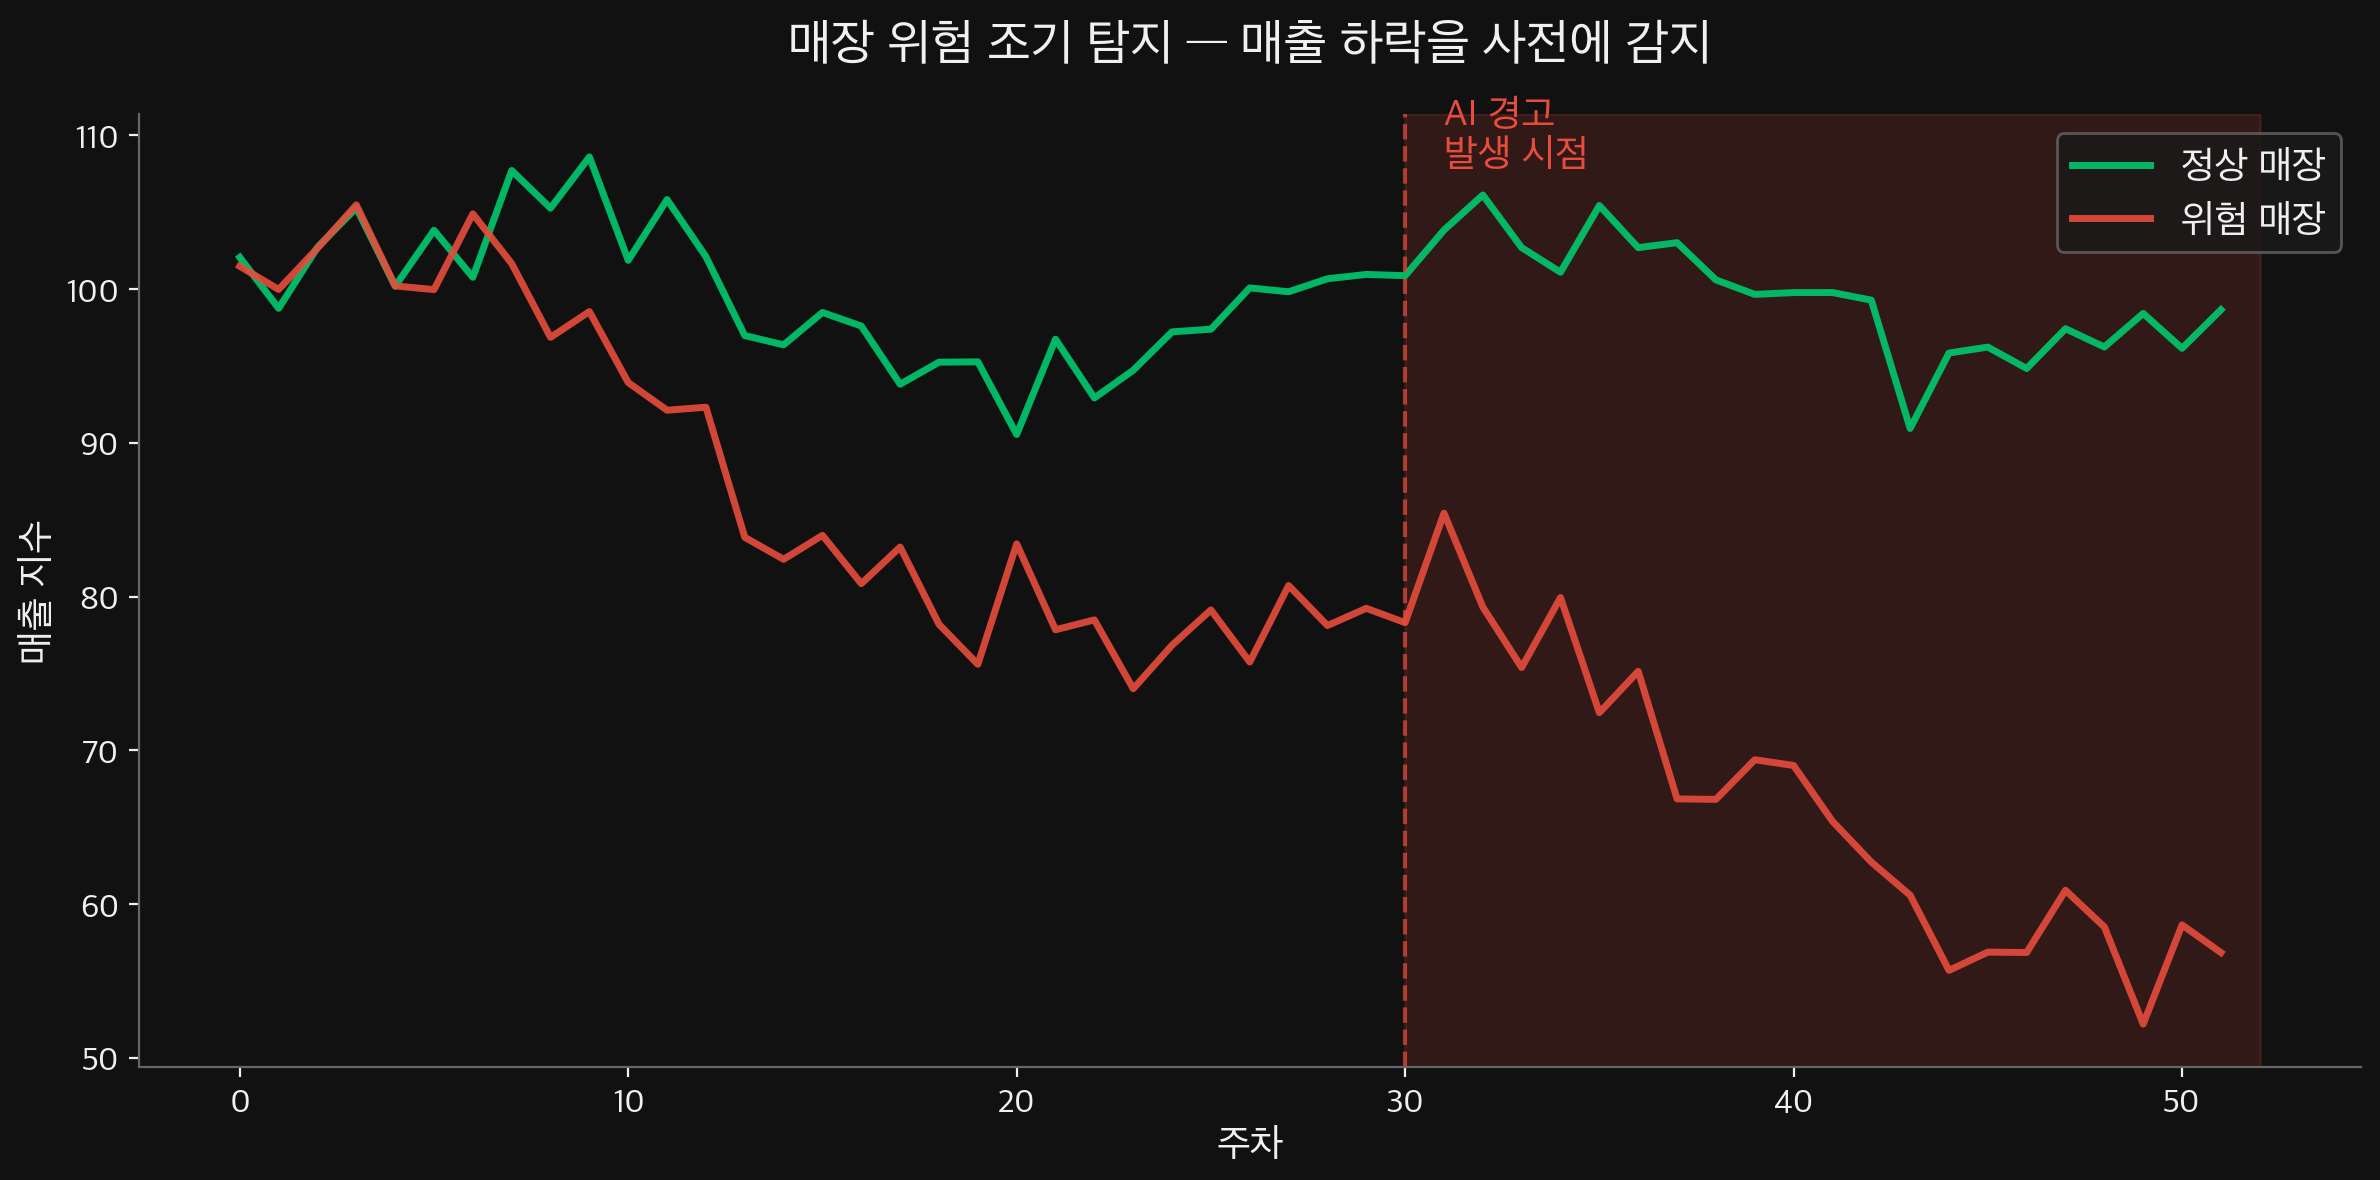
\includegraphics[width=0.85\textwidth]{v2_early_warning.png}
\caption{정상 매장 vs 위험 매장 — 하락 추세를 조기에 감지}
\end{figure}

\subsection{어떤 신호를 보는가}

\begin{itemize}[itemsep=6pt, leftmargin=2em]
  \item \textbf{특정 품목의 판매량 감소가 먼저 나타난다} — 전체 매출이 떨어지기 전에, 특정 카테고리(예: 신선식품)의 판매가 먼저 줄어드는 패턴
  \item \textbf{고객 수 변화} — 방문 고객 수의 감소는 매출 하락의 가장 강력한 선행 지표
  \item \textbf{장바구니 구성 변화} — 고객이 사는 품목의 다양성이 줄어들면 매장 이탈의 신호
\end{itemize}

\colorbox{lightblue}{%
\begin{minipage}{0.95\textwidth}\vspace{8pt}
\textbf{시사점:} 매출이 떨어진 후에 ``왜 떨어졌지?''를 분석하는 대신, AI가 \textbf{수개월 전에} ``이 매장 주의해야 합니다''라고 알려줍니다. 인력 재배치, 프로모션, 매장 리뉴얼 등의 \textbf{선제 대응}이 가능해집니다.
\vspace{8pt}
\end{minipage}%
}

\newpage

% ═══════════════════════════════════════════════════════
% 4. 원인 분석
% ═══════════════════════════════════════════════════════
\section{왜 안 팔리는지까지 알려줍니다}

매출이 떨어졌을 때, 가장 중요한 질문은 ``왜?''입니다.

\begin{table}[H]
\centering
\renewcommand{\arraystretch}{1.4}
\begin{tabularx}{\textwidth}{L{4cm} X L{4cm}}
\toprule
\rowcolor{lightblue} \textbf{원인} & \textbf{AI가 보는 신호} & \textbf{대응} \\
\midrule
\textbf{경쟁사 출점} & 반경 내 경쟁 매장 수 변화, 고객 이동 패턴 & 차별화 전략, 가격 대응 \\[6pt]
\textbf{고객 이탈} & 방문 고객 수 감소, 단골 비율 하락 & 타겟 프로모션, 로열티 프로그램 \\[6pt]
\textbf{구매 패턴 변화} & 장바구니 구성 변화, 특정 카테고리 감소 & 품목 재구성, MD 전략 수정 \\[6pt]
\textbf{계절/시기 효과} & 시계열 패턴, 전년 동기 대비 & 시즌별 발주 조정 \\[6pt]
\textbf{지역 인구 변화} & 상권 인구 추이, 연령대 변화 & 장기 전략 재검토 \\
\bottomrule
\end{tabularx}
\caption{매출 변동 원인 분석 체계}
\end{table}

AI 모델은 SHAP(Shapley Additive Explanations) 기법으로 \textbf{각 변수가 예측에 얼마나 기여했는지}를 정량적으로 분해합니다. ``이 매장의 매출이 떨어진 이유의 60\%는 고객 수 감소, 25\%는 장바구니 축소, 15\%는 계절 효과'' — 이런 수준의 분석이 가능합니다.

\newpage

% ═══════════════════════════════════════════════════════
% 5. 온라인과 오프라인은 다르게 관리해야 합니다
% ═══════════════════════════════════════════════════════
\section{온라인과 오프라인은 다르게 관리해야 합니다}

284개 매장 데이터를 분석한 결과, 가장 의외의 발견은 \textbf{온라인과 오프라인에서 매출을 결정하는 상품 분류 단위가 정반대}라는 것이었습니다.

\begin{figure}[H]
\centering
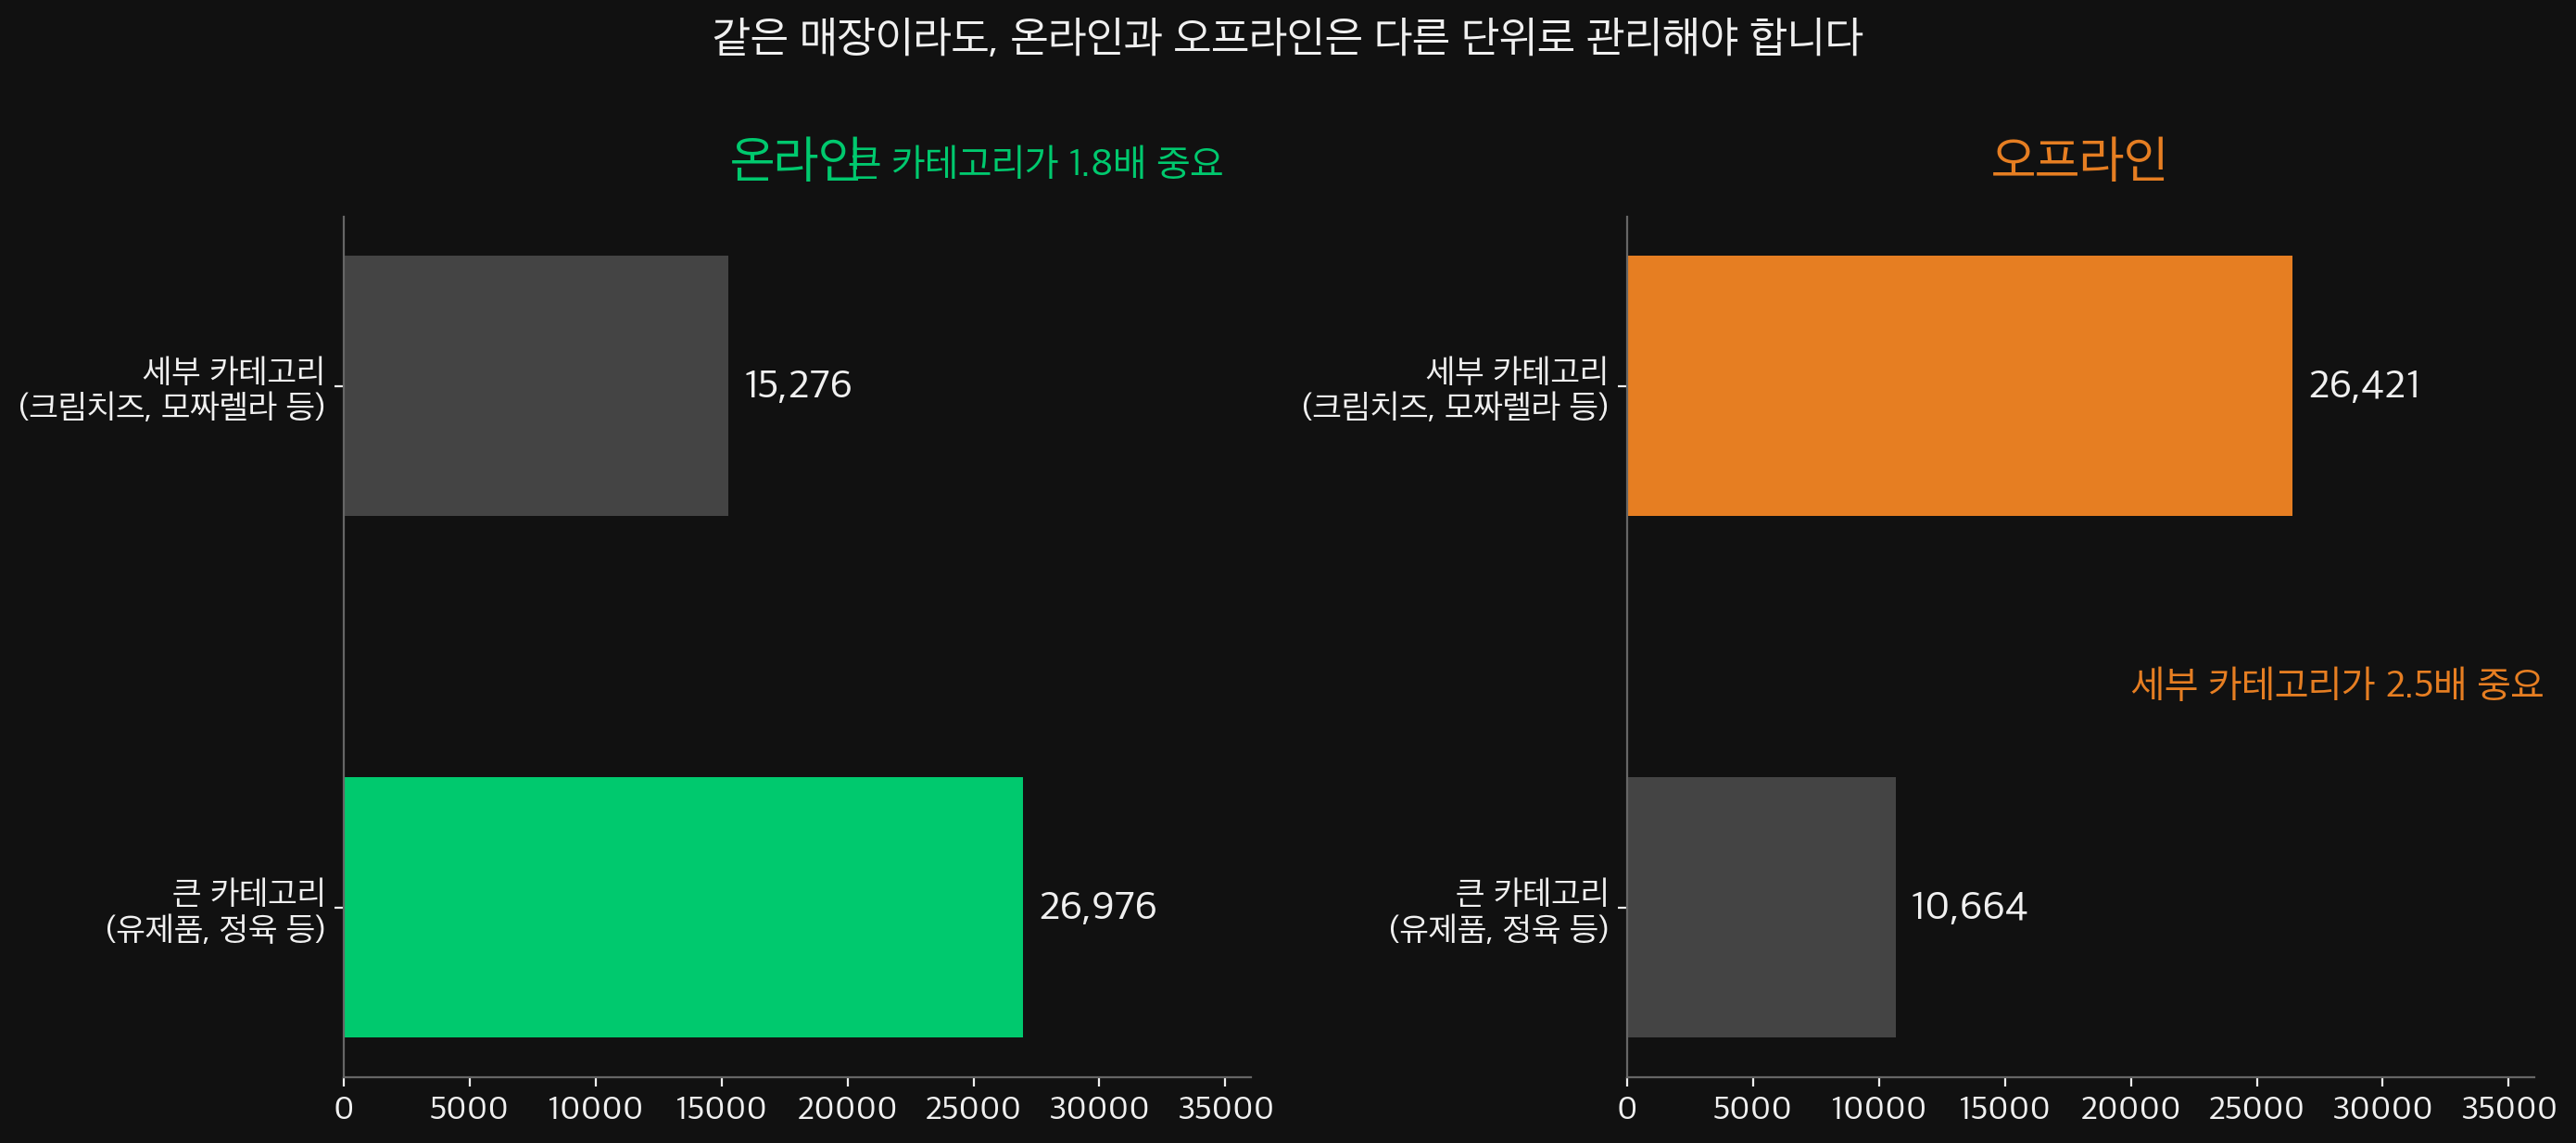
\includegraphics[width=0.9\textwidth]{v2_category_insight.png}
\caption{온라인: 큰 카테고리 중심 / 오프라인: 세부 카테고리 중심}
\end{figure}

\begin{table}[H]
\centering
\renewcommand{\arraystretch}{1.3}
\large
\begin{tabular}{L{4cm} L{5.5cm} L{5.5cm}}
\toprule
\rowcolor{lightblue} & \textbf{온라인} & \textbf{오프라인} \\
\midrule
\textbf{핵심 단위} & 큰 카테고리 (Class) & 세부 카테고리 (Subclass) \\[4pt]
\textbf{고객 행동} & ``유제품 3종, 과일 2종'' & ``크림치즈 vs 모짜렐라'' \\[4pt]
\textbf{쇼핑 방식} & 검색 → 필터 → 장바구니 & 보고 → 만지고 → 고르기 \\[4pt]
\textbf{관리 원칙} & \textcolor{darkblue}{\textbf{카테고리 구색 다양성}} & \textbf{세부 상품 진열 큐레이션} \\
\bottomrule
\end{tabular}
\end{table}

\colorbox{lightblue}{%
\begin{minipage}{0.95\textwidth}\vspace{8pt}
\textbf{실무 원칙:} 온라인 MD는 ``카테고리를 얼마나 다양하게 제공하는가''를 기준으로, 오프라인 MD는 ``어떤 세부 상품을 눈높이에 놓는가''를 기준으로 기획해야 합니다.\\[4pt]
이 결과는 4가지 서로 다른 모델 사양에서 \textbf{100\% 일관}되게 확인되었습니다.
\vspace{8pt}
\end{minipage}%
}

\newpage

% ═══════════════════════════════════════════════════════
% 6. 예측 정확도
% ═══════════════════════════════════════════════════════
\section{예측 정확도}

284개 슈퍼마켓 매장의 실제 거래 데이터로 구축하고, \textbf{학습에 사용하지 않은 미래 기간의 데이터}로만 검증한 결과입니다.

\begin{figure}[H]
\centering
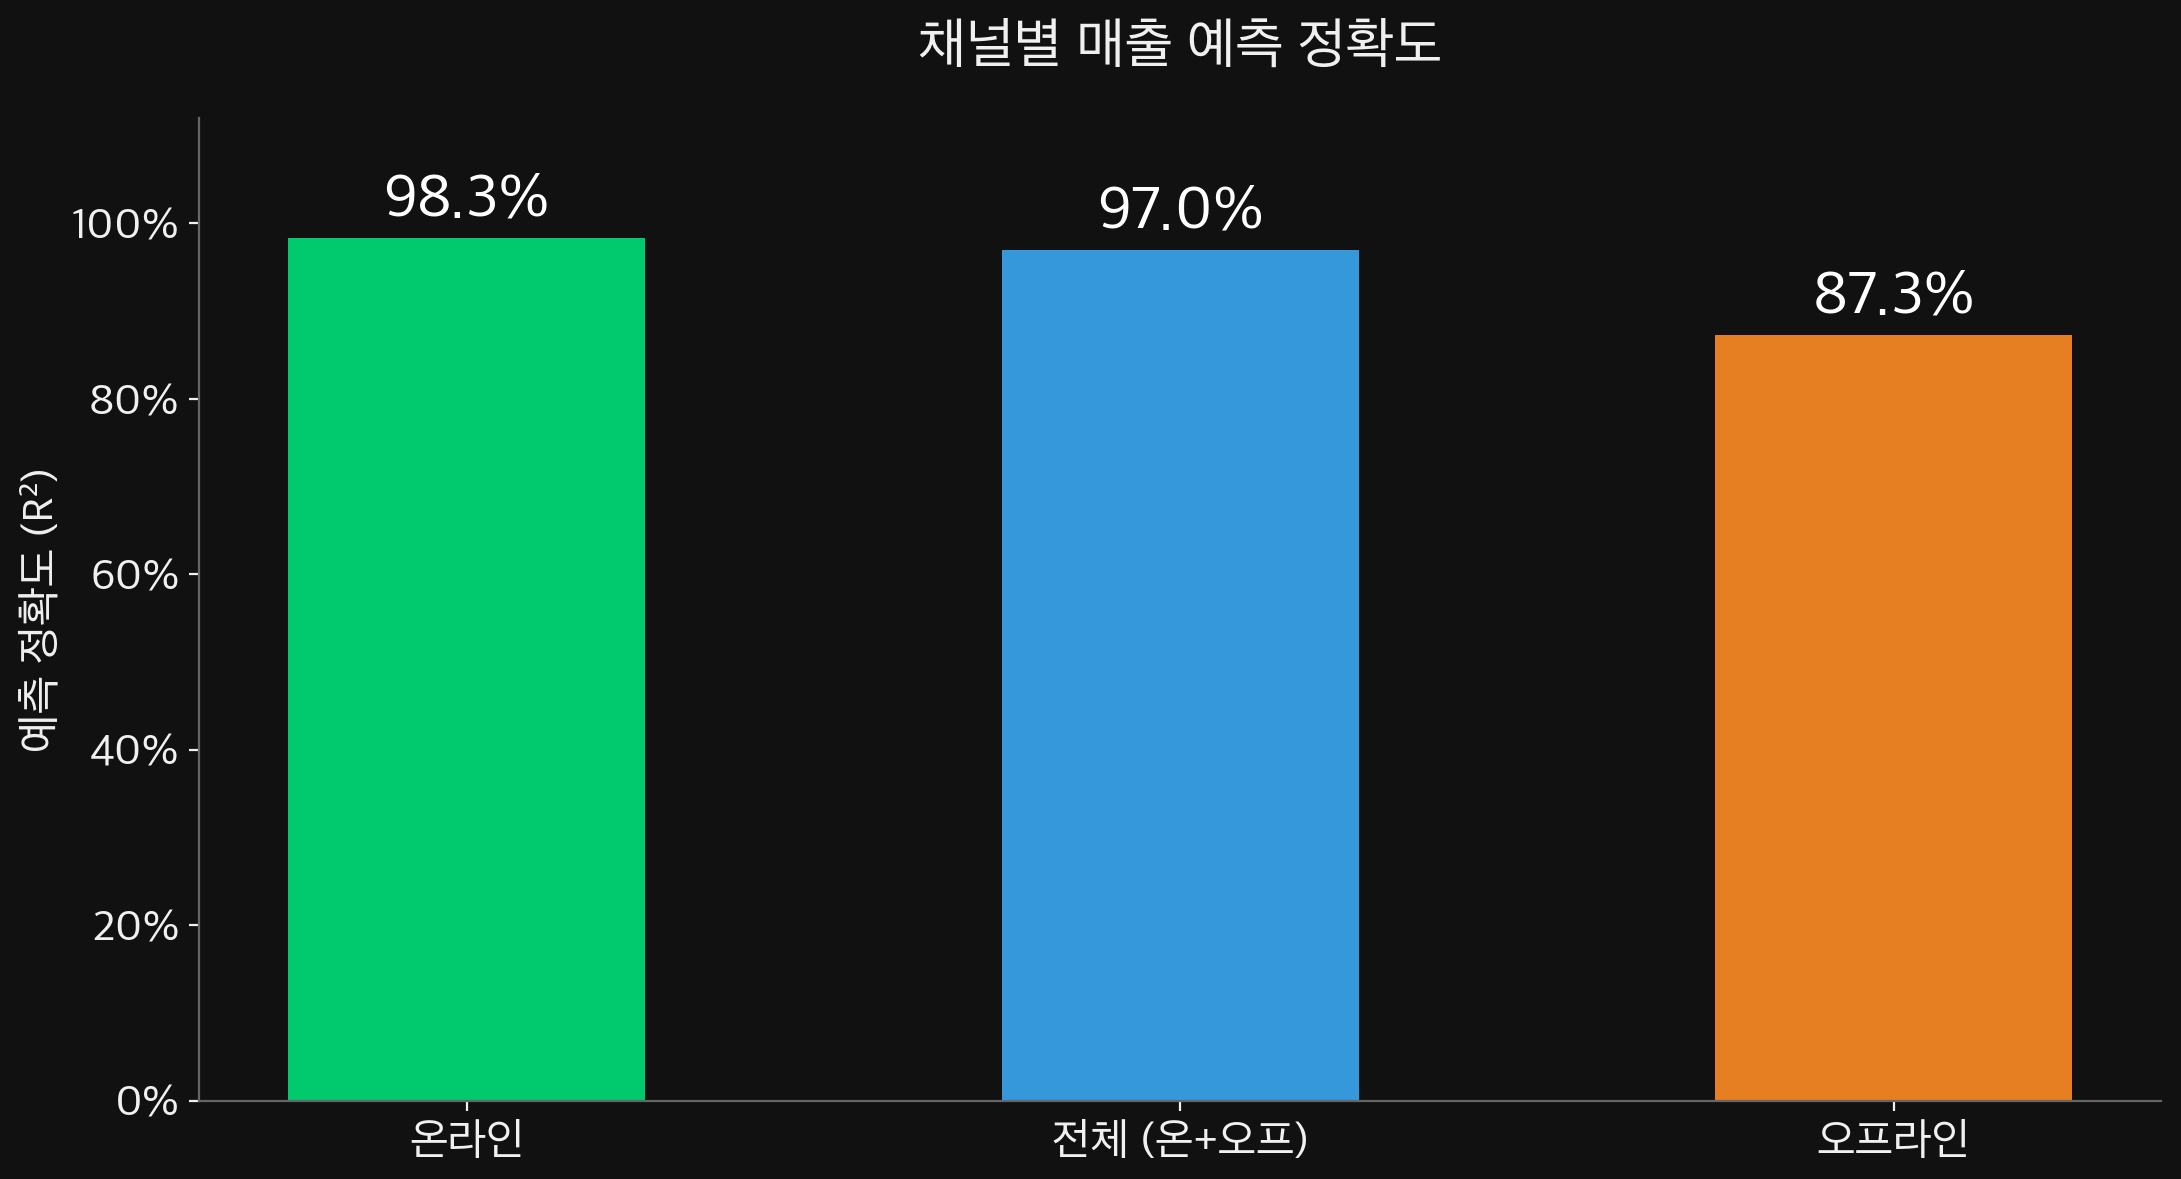
\includegraphics[width=0.8\textwidth]{v2_channel_accuracy.png}
\caption{채널별 매출 예측 정확도 (Out-of-sample, R²)}
\end{figure}

\begin{table}[H]
\centering
\large
\begin{tabular}{L{5cm} C{3cm} C{3cm} C{3cm}}
\toprule
\rowcolor{lightblue}  & \textbf{온라인} & \textbf{전체} & \textbf{오프라인} \\
\midrule
\textbf{예측 정확도 (R²)} & \textcolor{darkblue}{\textbf{98.3\%}} & \textbf{97.0\%} & 87.3\% \\[4pt]
검증 건수 & 2,560건 & 3,185건 & 3,057건 \\[4pt]
분석 매장 수 & 225개 & 284개 & 281개 \\
\bottomrule
\end{tabular}
\end{table}

오프라인 매출은 충동 구매, 날씨, 매장 환경 등 변수가 많아 예측 난이도가 높지만, 그래도 87\%의 설명력을 달성합니다. 데이터가 충분히 축적될수록 정확도는 더 올라갑니다.

\vspace{0.5cm}

\textbf{분석 방법:}
\begin{itemize}[itemsep=3pt, leftmargin=2em]
  \item XGBoost + LightGBM 앙상블 모델
  \item 149개 변수 (고객 구매 패턴, 상품 구성, 경쟁 환경, 시계열 추세 등)
  \item SHAP 기반 변수 중요도 해석 — ``왜 이런 예측이 나왔는지''까지 설명
\end{itemize}

\newpage

% ═══════════════════════════════════════════════════════
% 7. 연구실 소개
% ═══════════════════════════════════════════════════════
\section{한양대학교 빅데이터마케팅 랩}

\begin{table}[H]
\centering
\renewcommand{\arraystretch}{1.3}
\begin{tabularx}{\textwidth}{L{4cm} X}
\toprule
\rowcolor{lightblue} & \\
\midrule
\textbf{연구실} & 한양대학교 경영대학 빅데이터마케팅 랩 (BDM Lab) \\[4pt]
\textbf{교수} & 임보람 (Ph.D., UT Dallas / M.S., UT Austin) \\[4pt]
\textbf{전문 분야} & AI/ML 기반 매출·수요 예측, 소비자 행동 분석, 인과분석 \\[4pt]
\textbf{핵심 기술} & XGBoost/LightGBM 앙상블, SHAP 해석, 시계열 예측 \\[4pt]
\textbf{적용 업종} & 슈퍼마켓, 프랜차이즈, 리테일, 식음료 \\
\bottomrule
\end{tabularx}
\end{table}

\subsection{데이터만 있으면 됩니다}

\begin{itemize}[itemsep=6pt, leftmargin=2em]
  \item \textbf{필요한 것:} 매장별 일간 또는 주간 매출 데이터 (최소 6개월)
  \item \textbf{추가 분석 가능:} 품목별 거래 데이터, 고객 정보 (로열티카드 등)
  \item \textbf{외부 데이터 구매 불필요} — 자사 POS 데이터만으로 고정밀 예측 가능
\end{itemize}

\vspace{1.5cm}

\begin{center}
\textcolor{medblue}{\rule{8cm}{0.8pt}}

\vspace{1cm}

{\Large\bfseries\color{darkblue} 문의}

\vspace{0.5cm}

{\large\color{darkgray}
임보람 교수\\[4pt]
한양대학교 경영대학\\[4pt]
빅데이터마케팅 랩\\[8pt]
brlim@hanyang.ac.kr\\[4pt]
bigdatamarketinglab.com}
\end{center}

\end{document}
